\documentclass{sintefbeamer}

% packages, font, color, and newcommands
\usepackage{amsfonts, amsmath, oldgerm, lmodern, bm}
% \usepackage[font={footnotesize}]{caption}
\usepackage{natbib}
\usepackage{url}
\usepackage{tikz}
\usepackage{amssymb}
\usepackage{amsmath}
\usepackage{amsthm}
\usepackage{mathrsfs}
\usepackage{empheq}
\usepackage{mdframed}
\usepackage{bm}
\usepackage{animate}
\usepackage{xcolor,colortbl}
\usepackage{graphicx}
\usepackage{pgfplots}
\bibliographystyle{apalike}
\usefonttheme{serif}
\usetikzlibrary{calc}

% \title{Theoretical prediction of the Reynolds stress in low inertial buoyant emulsion.}
\title{Nearest particle statistics in rising monodisperse suspensions of drops.}
\subtitle{A theoretical study on pseudo turbulence}
\author{\href{https://scholar.google.com/citations?user=GQDBlaQAAAAJ&hl=en}{\underline{N. Fintzi}\footnote{IFP \'Energies Nouvelles, France}$^{,2}$}, JL. Pierson$^1$ and S. Popinet\footnote{Sorbonne Universit\'e, France}}
% \date{Created on May 22, 2022}

\titlebackground{image/800good.png}

% document body
\addtobeamertemplate{navigation symbols}{}{%
    \usebeamerfont{footline}%
    \usebeamercolor[fg]{footline}%
    % \hspace{1em}%
    % \vspace{1em}%
    \insertframenumber/\inserttotalframenumber
}
\usepackage{stmaryrd}

\usepackage{amsmath}


\begin{document}
\maketitle


\begin{frame}
  \frametitle{Industrial context}
  \underline{Buoyant emulsions are ubiquitous in chemical engineering processes :}
  \begin{itemize}
    \item Separation processes (gravity separators, flotation)
    \item Bubble column reactors
    \item Liquid-liquid separation
  \end{itemize}
  \vfill
  \pause
  \underline{In all those process we want to : }
  \begin{itemize}
    \item Predict global hydrodynamics using \textbf{Euler-Euler} framework. 
    \begin{itemize}
      \item Closure for the interphase drag forces, first moments of hydrodynamics forces, inter-particles forces.
      \item Closure of coalesce and break-up to predict the size distribution.
      \item Closure for the \textbf{Reynolds stress} or Pseudo-turbulent tensor :$\avg{\textbf{u}'\textbf{u}'}$.
      % \begin{itemize}
      %   \item Describe the interactions between pairs of droplets
      %   \item Predict interaction frequency
      %   \item Predict film drainage time 
      % \end{itemize}
    \end{itemize}
  \end{itemize}
\pause
  \vfill
$\to$ In this presentation we focus on the theoretical modeling of \textbf{Reynolds Stress}.
\end{frame}

\section{Introduction : what is the Reynolds stress ?}

\begin{frame}{To model the processes we use Euler-Euler framwork }
  Averaged \textbf{mass} and \textbf{momentum} equations for the continuous phase :
\begin{align*}
  % \phi_d + \phi_f &= 1\\
  \pddt (\phi_f \rho_f)  
  + \div (\phi_f \rho_f\textbf{u}_f)
  &= 
  0\\
  \pddt (\phi_f \rho_f\textbf{u}_f)  
  + \div (
      \phi_f \rho_f\textbf{u}_f\textbf{u}_f
      + \bm{\sigma}_f^\text{eff}
  )
  &= 
  \phi_f  \rho_f \textbf{g}
  + 
  \underbrace{
    \avg{\delta_I \bm{\sigma}_f^0 \cdot \textbf{n}_f}
  }_\text{Interphase force}
\end{align*}
With the effective stress : 
\begin{align*}
  &\bm{\sigma}_f^\text{eff}
  = 
   \underbrace{\rho_f\avg{\chi_f \textbf{u}_f'\textbf{u}_f'}}_\text{Reynolds stress}
    - \underbrace{\phi_f \bm{\sigma}_f}_\text{Newtonian stress}
\end{align*}
\begin{itemize}
  \item $\textbf{u}_f$ mean velocity of the continuous phase.  
  \item $\rho_f$ : density of the continuous phase. 
  \item $\phi_f$ : volume fraction of the continuous phase. 
  \item $\avg{\ldots}$ : the ensemble average operator. 
  \item $\textbf{u}_f' = \textbf{u}^0_f - \textbf{u}_f$ where $\textbf{u}_f^0$ is the local (non-averaged) fluid velocity. 
\end{itemize}
\end{frame}





\begin{frame}{Objectives and Hypothesis :}
  \begin{equation*}
     \avg{\chi_f \textbf{u}_f'\textbf{u}_f'}
     = 
     \text{Particle induced turbulence}
     + \text{Single phase turbulence}
  \end{equation*}
  \hrule\hrule
  \pause
  \begin{itemize}
    \item 
    Focus on the \textbf{Particle induced turbulence}. 
    \item Assuming : 
    \begin{itemize}
      \item Negligible inertia (\textbf{Stokes} regime)
      \item Dilute regime such that $\phi^{2} \approx 0$ 
      \item Mono-disperse suspension of droplets of radius $a$
    \end{itemize}
  \end{itemize}
\hrule\hrule
  \pause
  In this specific situation we can write  (Bachelor 1972) :
  \begin{equation*}
    \avg{\chi_f \textbf{u}'_f\textbf{u}'_f}(\textbf{x},t)
    = 
    n_p(\textbf{x},t)
    \int_{|\textbf{r}| > a }
     \textbf{u}^1\textbf{u}^1(\textbf{r}|\textbf{x}) d\textbf{r}
    +\mathcal{O}(\phi^2)
\end{equation*}

\begin{itemize}
  \item $\phi$ : dispersed phase volume fraction.
  \item $n_p = \frac{3\phi}{4\pi a^3}$ : number density of particles ;
  \item $\textbf{u}^1(\textbf{r}|\textbf{x})$ : disturbance field evaluated at \textbf{r} produced by a droplet located at \textbf{x}. 
\end{itemize}
\end{frame}


\begin{frame}
  \frametitle{L.Van Wijngaarden approach for potential flow.}

  \begin{columns}
    \column{0.8\textwidth}
Disturbance velocity field of an isolated translating bubble is :
\begin{equation*}
  \textbf{u}'_\text{pot}(\textbf{r})
  = \frac{a^3 \textbf{U}}{2} \cdot \left(\frac{\textbf{I}}{r^3} - \frac{3 \textbf{rr}}{r^5}\right)
  \text{    for    }r>a
\end{equation*}
\column{0.2\textwidth}
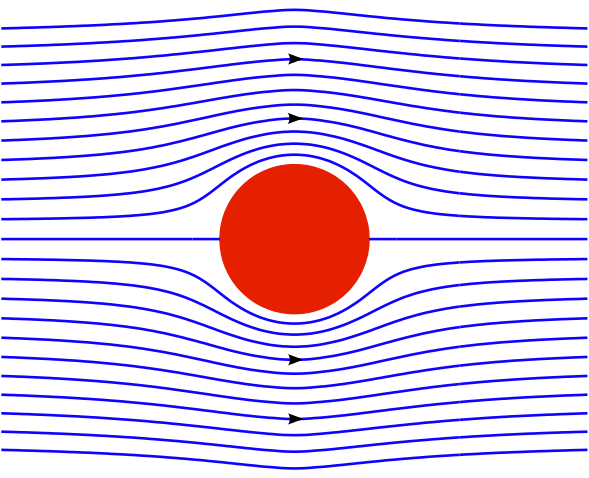
\includegraphics[width=\textwidth,angle=90]{image/Potential_cylinder.png}
\end{columns}
\pause
Therefore, the Reynolds stress approximation in homogeneous dilute suspension of spherical bubbles can be written Wijngaarden(1976): 
  \begin{align*}
    \avg{\chi_f \textbf{u}'_f\textbf{u}'_f}(\textbf{x},t)
    =
    n_p(\textbf{x},t)
      \int_{|\textbf{r}| > a }
       \textbf{u}_\text{pot}\textbf{u}_\text{pot}(\textbf{r}|\textbf{x}) d\textbf{r}
    = \phi \left(\frac{3}{20} U^2\textbf{I} + \frac{1}{20}\textbf{UU} \right)
\end{align*}

  \begin{itemize}
    \item $\phi$ is the volume fraction of the dispersed phase. 
    \item $\textbf{U} = \textbf{u}_f-\textbf{u}_p$ is the relative velocity between phases. 
    \item The integral converge because $\textbf{u}_\text{pot}  \sim r^{-3}$
  \end{itemize}
  \underline{$\to$ We aim for the same closure but in Stokes regime}
\end{frame}


\begin{frame}
  \frametitle{Can we do the same but for Stokes flow ?}
  The stokes flow solution of an isolated translating drop is :
  \begin{columns}
    \column{0.6\textwidth}
  \begin{multline*}
    \textbf{u}_\text{stokes} 
    = \left(\frac{ \textbf{I}}{r} + \frac{\textbf{rr}}{r^3}\right)  \frac{1}{4}\left(\frac{3\lambda + 2}{\lambda +1}\right) a \cdot \textbf{U}\\
    - \left(-\frac{\textbf{I}}{r^3} + \frac{3 \textbf{rr} }{r^5}\right)  \frac{1}{4}\left(\frac{\lambda}{\lambda +1}\right) a^3 \cdot \textbf{U}
  \end{multline*}
  \begin{itemize}
      \item $\lambda$ is the viscosity ratio.
  \end{itemize}
  \column{0.3\textwidth}
  \begin{figure}
    % \caption{Disturbance velocity field of an isolated translating spherical droplet}
    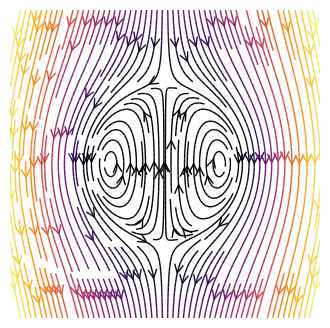
\includegraphics[width=\textwidth]{image/Rising_Stokes.png}
  \end{figure}
  \end{columns}
\pause
  In this case : 
  \begin{align*}
    \avg{\chi_f \textbf{u}'_f\textbf{u}'_f}(\textbf{x},t) / n_p
    &\approx 
    \int_{|\textbf{r}| > a} \textbf{u}'_\text{stokes}\textbf{u}'_\text{stokes}   d\textbf{r}
    % - \phi_f \textbf{u}_f\textbf{u}_f
    =\infty 
  \end{align*}
  \underline{\textbf{The integral diverges}  ! (beacause $\textbf{u}_\text{stokes} \sim r^{-1}$).}
\end{frame}
\begin{frame}
  \frametitle{Why does the integral diverges ?}

  Batchelor (1972)'s  formula:
  \begin{equation*}
    \avg{\chi_f \textbf{u}'_f\textbf{u}'_f}(\textbf{x},t)
    = 
    n_p(\textbf{x},t)
    \int_{|\textbf{r}| > a }
     \textbf{u}^1\textbf{u}^1(\textbf{r}|\textbf{x}) d\textbf{r}
    +\mathcal{O}(\phi^2)
\end{equation*}

  Batchelor (1972)'s  formula \underline{without approximation}: 
  \begin{equation}
    \avg{\chi_f \textbf{u}_f' \textbf{u}_f'}[\textbf{x},t] =
    % \int_{\mathbb{R}^6}
    % \avg{\delta_1\chi_f \textbf{u}_f' \textbf{u}_f'}[\textbf{x},t]
    % d\textbf{y}
    % d\textbf{w}\\
    % &= 
    \int_{|\textbf{r}| > a } \textbf{u}^1\textbf{u}^1(\textbf{r}|\textbf{x}) d\textbf{r}
    % + 
    % \int_{\mathbb{R}^6}
    % \avg{\delta_1 \chi_f\textbf{u}_f'' \textbf{u}_f''}
    % d\textbf{y}
    % d\textbf{w}
    + Error
  \end{equation}
  \begin{equation}
    Error = \int_{|\textbf{r}| > a }    
    \textcolor{red}{
    \mathcal{O}(\textbf{u}^1
    \textbf{u}^1 \times |\textbf{r}|)}
    d\textbf{r}
  \end{equation}


$\to$ We conclude that this method is unable to provide physical result when $\textbf{u}^1 \sim \mathcal{O}(r^{-1})$, since in this case the \text{Error} term is infinite. 

$\to$ Since the problem is purely mathematical, we can find a solution using a more ``accurate'' method.

\end{frame}

\begin{frame}
  {Going further}
   Model for \textbf{Drops induced dissipation rate} : 
   \begin{multline*}
    \avg{\chi_f \bm\sigma_f^0 :\grad\textbf{u}_f^0}
    =
    \frac{3\mu_f \phi_d}{2a^2}
    \frac{(3\lambda^2 + 4\lambda +2)}{(\lambda + 1)^2}
    (\textbf{u}_{fp}\cdot \textbf{u}_{fp} + 2 \avg{\textbf{u}_p'\cdot\textbf{u}_p'}) \\
    + 
    \frac{3\mu_f \phi_d}{5}
    \frac{(5\lambda^2 + 4\lambda +4)}{(\lambda + 1)^2}
    \textbf{E}:\textbf{E}
    +2 \phi_f \textbf{E}:\textbf{E}
\end{multline*}
\end{frame}



\section{The Nearest Particle Statistics}

\begin{frame}{The Nearest Particle Statistics (NPS) approach (DZ Zhang, JFM, 2020) Definition}
  \begin{align*}
    \phi_f[\textbf{x},t] &= \avg{\chi_f[\textbf{x},\FF,t]}\\
    (\phi_f \textbf{u}_f)[\textbf{x},t] &= \avg{(\textbf{u}_f^0\chi_f)[\textbf{x},\FF,t]}\\
    P_\text{nst}[\textbf{r}|\textbf{x},t]\phi_f[\textbf{x},t] &= \avg{\chi_f[\textbf{x},\FF,t]\sum_i^N \delta(\textbf{x}_i[\FF,t] - \textbf{x} - \textbf{r}) h_i[\textbf{x},t,\FF]}\\
    \textbf{u}_f^\text{nst}[\textbf{r},\textbf{x},t] P_\text{nst}[\textbf{r}|\textbf{x},t]\phi_f[\textbf{x},t] &= \avg{(\textbf{u}_f^0\chi_f)[\textbf{x},\FF,t]\sum_i^N \delta(\textbf{x}_i[\FF,t] - \textbf{x} - \textbf{r}) h_i[\textbf{x},t,\FF]}
  \end{align*}
  \begin{itemize}
    \item $\FF$ random realization of the flow. 
    \item $\textbf{u}_f^0$ non-averaged local fluid velocity, at \textbf{x} and $t$ for the configuration $\FF$.
    \item $\chi_f$ phase indicator function of the fluid.
    \item $\textbf{u}_f$ ensemble averaged fluid velocity, at \textbf{x} and $t$.
    \item $h_i[\textbf{x},t] = 1$ if the nearest neighbor to \textbf{x} is the particle $i$, 0 otherwise.  
  \end{itemize}
\end{frame}
\begin{frame}{The Nearest Particle Statistics (NPS) approach (DZ Zhang, JFM, 2020) Definition}
  \begin{align*}
    \avg{\chi_f \textbf{u}_f'\textbf{u}_f'}
    &=
    \int 
    \avg{(\textbf{u}_f^0\textbf{u}_f^0\chi_f)[\textbf{x},\FF,t]\sum_i^N \delta(\textbf{x}_i[\FF,t] - \textbf{x} - \textbf{r}) h_i[\textbf{x},t,\FF]} 
    d\textbf{r} \\
    &=\phi_f
    \underbrace{\int 
      \textbf{u}^\text{nst}_f
      \textbf{u}^\text{nst}_f 
      P_\text{nst}(\textbf{r}|\textbf{x}) d\textbf{r} 
    }_\text{Averaged wake contribution}
    + \underbrace{ 
      \int \avg{\delta_i h_i \chi_f \textbf{v}_f''\textbf{v}_f''}  d\textbf{r}
    % P_{nst}(\textbf{x},t,\textbf{r}) d\textbf{r}
    }_{\mathcal{O}(\phi^2)}
  \end{align*}

  \begin{itemize}
    \item $\textbf{v}^\text{nst}(\textbf{x}|\textbf{y})$ disturbance velocity evaluated at \textbf{x}, averaged on every configuration where the nearest particle to the point \textbf{x} is located at $\textbf{x} + \textbf{r}$. 
    \item $\textbf{v}''_f = \textbf{u}^0_f - \textbf{u}^\text{nst}_f$ fluctuating values of the local velocity $\textbf{u}_f^0$ (non-averaged) around $\textbf{u}_f^\text{nst}$.
    \item $P_\text{nst}(\textbf{r}|\textbf{x})$ is the probability of finding a nearest particle at \textbf{r} knowing \textbf{x} is occupied by the continuous phase.   
    \item This relation is exact and require no assumption. 
  \end{itemize}
\end{frame}

\begin{frame}{The Nearest Particle Statistics (NPS) approach (DZ Zhang, JFM, 2020)}
  Using the relation between ensemble average $\avg{\ldots}$ and NPS average we obtain :
  \begin{equation*}
    \avg{\chi_f \textbf{u}'_f\textbf{u}'_f}[\textbf{x},t]
    = \phi_f
    \underbrace{\int 
      \textbf{u}^\text{nst}_f
      \textbf{u}^\text{nst}_f 
      P_\text{nst}(\textbf{r}|\textbf{x}) d\textbf{r} 
    }_\text{Averaged wake contribution}
    + \underbrace{ 
      \int \avg{\delta_i h_i \chi_f \textbf{v}_f''\textbf{v}_f''}  d\textbf{r}
    % P_{nst}(\textbf{x},t,\textbf{r}) d\textbf{r}
    }_{\mathcal{O}(\phi^2)}
  \end{equation*}

\begin{itemize}
  \item $\textbf{v}^\text{nst}(\textbf{x}|\textbf{y})$ disturbance velocity evaluated at \textbf{x}, averaged on every configuration where the nearest particle to the point \textbf{x} is located at $\textbf{x} + \textbf{r}$. 
  \item $\textbf{v}''_f = \textbf{u}^0_f - \textbf{u}^\text{nst}_f$ fluctuating values of the local velocity $\textbf{u}_f^0$ (non-averaged) around $\textbf{u}_f^\text{nst}$.
  \item $P_\text{nst}(\textbf{r}|\textbf{x})$ is the probability of finding a nearest particle at \textbf{r} knowing \textbf{x} is occupied by the continuous phase.   
  \item This relation is exact and require no assumption. 
\end{itemize}
\end{frame}


\begin{frame}
  \frametitle{Graphical representation of $\textbf{u}_f^\text{nst}$ and $P_\text{nst}$ }
  \begin{equation*}
    \avg{\chi_f \textbf{u}'_f\textbf{u}'_f}[\textbf{x},t]
        = \phi_f\underbrace{\int 
      \textbf{u}^\text{nst}_f
      \textbf{u}^\text{nst}_f 
      P_\text{nst}(\textbf{r}|\textbf{x}) d\textbf{r} 
    }_\text{Averaged wake contribution}
    + \underbrace{ 
      \int \avg{\delta_i h_i \chi_f \textbf{v}_f''\textbf{v}_f''}  d\textbf{r}
    % P_{nst}(\textbf{x},t,\textbf{r}) d\textbf{r}
    }_{\mathcal{O}(\phi^2)}
  \end{equation*}
  \centering
  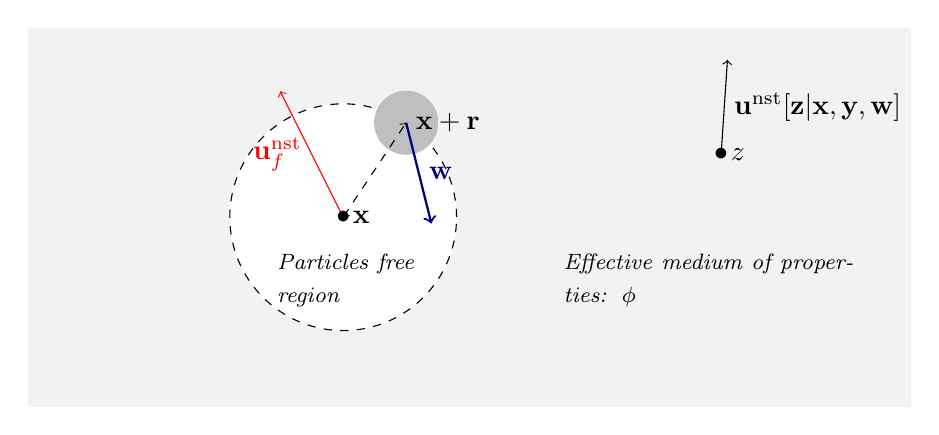
\begin{tikzpicture}[scale=0.8]
    \filldraw[gray!10](-5,-3) rectangle(9,3);
    \filldraw[white](0,0) circle (1.8);
    \filldraw[ gray!10!white](+2.6,0.5)circle (0.5);
    \filldraw[ gray!10!white](-1.5,2.2)circle (0.5);
    \draw[dashed](0:1.8) arc (0:360:1.8);
    % \filldraw[ gray!50!white](0,0) circle (0.5);
    \filldraw[ gray!50!white](1,1.5)circle (0.5);
    \filldraw[ gray!10!white](-0.2,2.5)circle (0.5);
    \draw[->,red](0,0)--++(-1,2)node[midway,left]{$\textbf{u}_f^\text{nst}$};
    \draw(0,0)node{$\bullet$}node[right]{$\textbf{x}$};
    \draw[dashed,<->](0,0)--(1,1.5)node[right]{$\textbf{x}+\textbf{r}$};
    \draw[->,blue!50!black,thick](1,1.5)--++(0.4,-1.6)node[midway,right]{$\textbf{w}$};
    % \draw[dashed](-0.2,3.5);
    \node[text width=2cm] (title) at (0.2,-1) {\footnotesize\textit{Particles free region}};
    % \node[ultra thick] (title) at (-0.5,-1.5) {(\textit{Case 1})};
    \node[text width=4cm] (title) at (6,-1) {\footnotesize\textit{Effective medium of properties:} $\phi$};
    \draw[->] (6,1)node{$\bullet$}node[right]{$z$}--++(0.1,1.5)node[right,midway]{$\textbf{u}^\text{nst}[\textbf{z}|\textbf{x},\textbf{y},\textbf{w}]$};
\end{tikzpicture} 
  

\end{frame}

\transwipe[direction=90]
\begin{frame}{The Nearest Particle Statistics (NPS) approach (DZ Zhang, JFM, 2020)}
  $P_\text{nst}(\textbf{r}|\textbf{x})$ is the probability of finding a nearest particle at \textbf{r} knowing \textbf{x} is occupied by the continuous phase.   

  In the dilute, isotropic and homogeneous regime : 
  \begin{equation*}
    \boxed{P_\text{nst}(\textbf{r}|\textbf{x})
    = \frac{3\phi}{4\pi}
    e^{ - \phi (|\textbf{r}|^3 - 1) }
    \text{ for }
    |\textbf{r}| > a }
  \end{equation*}
  \pause
\begin{columns}
  \column{0.5\textwidth}
  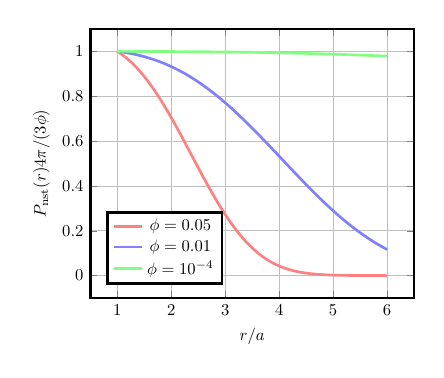
\begin{tikzpicture}[scale=0.6]
    \begin{axis}[
        xlabel={$r/a$},
        ylabel={$P_\text{nst}(r) 4\pi/ (3\phi) $},
        legend style={at={(0.05,0.05)}, anchor=south west},
        grid=major,
        domain=1:6,
        samples=100,
        ultra thick
    ]
    
    % Plot for phi = 0.05
    \addplot[color=red!50,ultra thick]
    { exp(-0.05 * (x^3 - 1))};
    \addlegendentry{$\phi = 0.05$}
    
    % Plot for phi = 0.01
    \addplot[color=blue!50,ultra thick]
    { exp(-0.01 * (x^3 - 1))};
    \addlegendentry{$\phi = 0.01$}
    
    % Plot for phi = 0.001
    \addplot[color=green!50,ultra thick]
    { exp(-0.0001 * (x^3 - 1))};
    \addlegendentry{$\phi = 10^{-4}$}
    
    \end{axis}
\end{tikzpicture}
\column{0.5\textwidth}
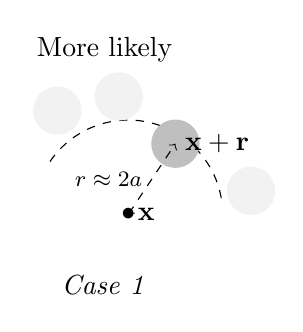
\begin{tikzpicture}[scale=0.6]
  \filldraw[ gray!10!white](+2.6,0.5)circle (0.5);
  \filldraw[ gray!10!white](-1.5,2.2)circle (0.5);
  \draw[dashed](10:2) arc (10:150:2);
  % \filldraw[ gray!50!white](0,0) circle (0.5);
  \filldraw[ gray!50!white](1,1.5)circle (0.5);
  \filldraw[ gray!10!white](-0.2,2.5)circle (0.5);
  \draw(0,0)node{$\bullet$}node[right]{$\textbf{x}$};
  \draw[dashed,<->](0,0)--(1,1.5)node[midway,left]{\footnotesize $r\approx 2 a$}node[right]{$\textbf{x}+\textbf{r}$};
  % \draw[dashed](-0.2,3.5);
  \node[ultra thick] (title) at (-0.5,3.5) {{More likely}};
  \node[ultra thick] (title) at (-0.5,-1.5) {\textit{Case 1}};
\end{tikzpicture} 
\hfill
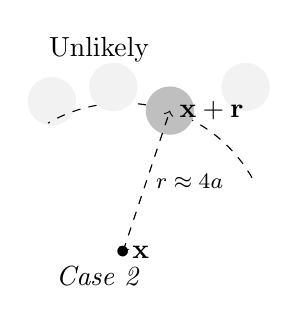
\begin{tikzpicture}[scale=0.6]
  \filldraw[ gray!10!white](+2.6,3.5)circle (0.5);
  \filldraw[ gray!10!white](-1.5,3.2)circle (0.5);
  \draw[dashed](30:3.16) arc (30:120:3.16);
  % \filldraw[ gray!50!white](0,0) circle (0.5);
  \filldraw[ gray!50!white](1,3)circle (0.5);
  \filldraw[ gray!10!white](-0.2,3.5)circle (0.5);
  \draw(0,0)node{$\bullet$}node[right]{$\textbf{x}$};
  \draw[dashed,<->](0,0)--(1,3)node[midway,right]{\footnotesize  $r\approx 4a$}node[right]{$\textbf{x}+\textbf{r}$};
  % \draw[dashed](-0.2,3.5);
  \node[ultra thick] (title) at (-0.5,4.3) {{Unlikely}};
  \node[ultra thick] (title) at (-0.5,-0.5) {\textit{Case 2}};
\end{tikzpicture} 


\end{columns}

\end{frame}


\begin{frame}
  \frametitle{How to find the nearest neighbor velocity field $\textbf{u}_f^{nst}$ ? }
  \centering
  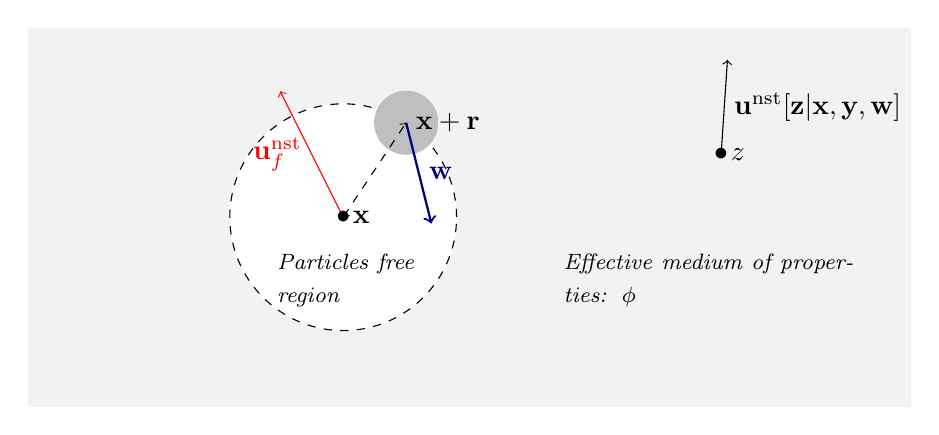
\begin{tikzpicture}[scale=0.8]
    \filldraw[gray!10](-5,-3) rectangle(9,3);
    \filldraw[white](0,0) circle (1.8);
    \filldraw[ gray!10!white](+2.6,0.5)circle (0.5);
    \filldraw[ gray!10!white](-1.5,2.2)circle (0.5);
    \draw[dashed](0:1.8) arc (0:360:1.8);
    % \filldraw[ gray!50!white](0,0) circle (0.5);
    \filldraw[ gray!50!white](1,1.5)circle (0.5);
    \filldraw[ gray!10!white](-0.2,2.5)circle (0.5);
    \draw[->,red](0,0)--++(-1,2)node[midway,left]{$\textbf{u}_f^\text{nst}$};
    \draw(0,0)node{$\bullet$}node[right]{$\textbf{x}$};
    \draw[dashed,<->](0,0)--(1,1.5)node[right]{$\textbf{x}+\textbf{r}$};
    \draw[->,blue!50!black,thick](1,1.5)--++(0.4,-1.6)node[midway,right]{$\textbf{w}$};
    % \draw[dashed](-0.2,3.5);
    \node[text width=2cm] (title) at (0.2,-1) {\footnotesize\textit{Particles free region}};
    % \node[ultra thick] (title) at (-0.5,-1.5) {(\textit{Case 1})};
    \node[text width=4cm] (title) at (6,-1) {\footnotesize\textit{Effective medium of properties:} $\phi$};
    \draw[->] (6,1)node{$\bullet$}node[right]{$z$}--++(0.1,1.5)node[right,midway]{$\textbf{u}^\text{nst}[\textbf{z}|\textbf{x},\textbf{y},\textbf{w}]$};
\end{tikzpicture} 

  Conditionally averaging the stokes equations at a point \textbf{z}, knowing the fluid is present at \textbf{x} with its nearest neighbor at \textbf{y}, yields, 
  \begin{equation*}
    % \pddt \avg{(\delta_\text{nst-f} - P_\text{nst-f})\chi_f}
    \grad \cdot \textbf{u}^\text{nst}
    = 0
    \label{eq:mass_nst_d_stokes}
\end{equation*}
\begin{equation*}
    - \grad p^\text{nst} 
    + \mu_f \grad^2 \textbf{u}^\text{nst}
    = 
    \underbrace{\phi
    \textbf{g}
    \Delta\rho H(|\textbf{r}| - |\textbf{z} - \textbf{x}|)}_\text{particle-free zone buoyancy}
    + \underbrace{\frac{\textbf{w} \mu_f}{a^2} (1 +\grad^2) \delta(\textbf{x}+ \textbf{r} - \textbf{z})}_\text{point forces}
    \label{eq:momentum_nst_d_stokes}
\end{equation*}

\end{frame}

\begin{frame}
  \frametitle{How to find the nearest neighbor velocity field $\textbf{u}_f^{nst}$ ? }

  Conditionally averaging the stokes equations at a point \textbf{z}, knowing the fluid is present at \textbf{x} with its nearest neighbor at \textbf{y}, yields, 
  \begin{equation*}
    % \pddt \avg{(\delta_\text{nst-f} - P_\text{nst-f})\chi_f}
    \grad \cdot \textbf{u}^\text{nst}
    = 0
    \label{eq:mass_nst_d_stokes}
\end{equation*}
\begin{equation*}
    - \grad p^\text{nst} 
    + \mu_f \grad^2 \textbf{u}^\text{nst}
    = 
    \phi
    \textbf{g}
    \Delta\rho H(|\textbf{y} - \textbf{x}| - |\textbf{z} - \textbf{x}|)
    + \frac{\textbf{w} \mu_f}{a^2} (\delta(\textbf{x} - \textbf{y}) +\grad^2\delta)
    \label{eq:momentum_nst_d_stokes}
\end{equation*}

\textbf{The solution : } 
\begin{equation}
  \frac{\textbf{v}^\text{nst}_f}{U}
  =
  \underbrace{\left(\frac{2+3\lambda}{4(1+\lambda)}\right)\textbf{U}\cdot\left[
      1
      +
      \frac{\lambda}{2(2+3\lambda)}\grad^2 
  \right]\mathcal{G}(\textbf{x},\textbf{y})}_\text{particle wake}
  + \underbrace{\phi A |\textbf{x}-\textbf{y}|^2 \textbf{k}}_\text{downstream flow}
  % + \mathcal{O}(\phi). 
  \label{eq:v_nst_solution_adim}
\end{equation}
\begin{equation*}
  \mathcal{G}(\textbf{r})
  = \frac{\bm\delta}{r}
  + \frac{\textbf{rr}}{r^3},
\end{equation*}
\begin{align*}
  \textbf{U} = \textbf{w} - \textbf{u}_f/U
  && 
  \textbf{k} = \textbf{g}/|\textbf{g}|
  &&
  A = \frac{Ga^2}{12 Re}=\frac{\Delta \rho g (2a)^2}{12 \mu_f U}
  \label{eq:A_general}
\end{align*}
\end{frame}

\begin{frame}
  \frametitle{Flow lines around a non-isolated droplet}
  \begin{figure}[h!]
    \centering
    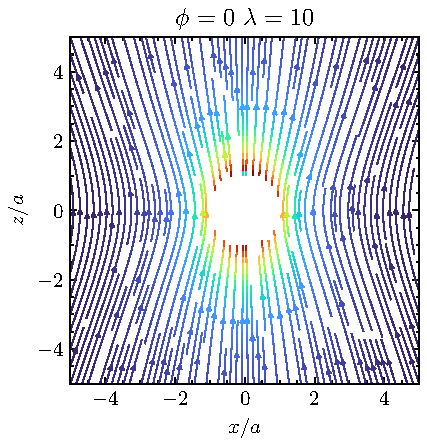
\includegraphics[height = 0.33\textwidth]{image/Vnst_l_10_0.pdf}
    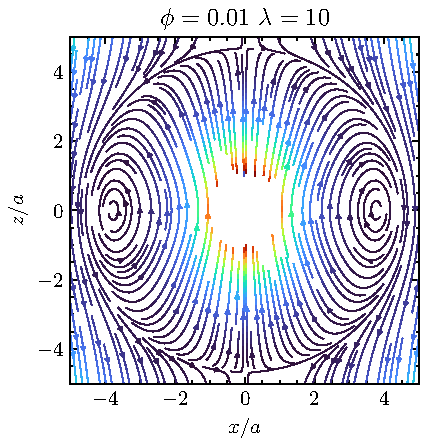
\includegraphics[height = 0.33\textwidth]{image/Vnst_l_10_1.pdf}
    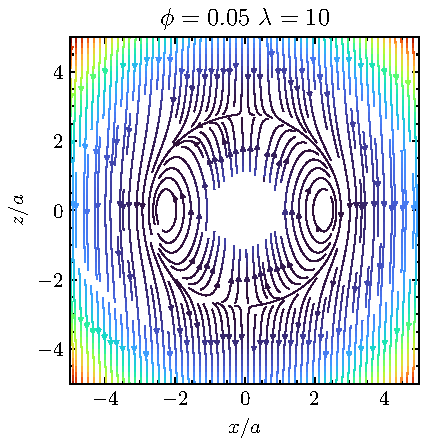
\includegraphics[height = 0.33\textwidth]{image/Vnst_l_10_5.pdf}
    % 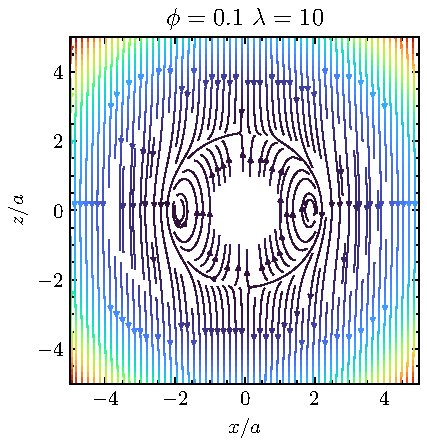
\includegraphics[height = 0.33\textwidth]{image/Vnst_l_10_10.pdf}
    \caption{Streamlines of the disturbance velocity field $\textbf{u}^\text{nst}_f(\textbf{r}_f)$ \eqref{eq:v_nst_solution_adim}  in the cross-section given by the plane $(\textbf{e}_x,\textbf{e}_z)$, for multiples volume fraction $\phi = 0, 0.01$ and $0.05$ at $\lambda = 10$.  
    The color map indicates the magnitude of the velocity, from black which corresponds to a velocity magnitude of 0, to the color at the interface which corresponds to 1.
    In this situation $\textbf{e} = \textbf{e}_z$ and $\textbf{k} = -\textbf{e}_z$}
    \label{fig:vnst_vertical}
\end{figure}
  

\end{frame}
\begin{frame}
  \frametitle{Flow lines around a non-isolated droplet}
  \begin{figure}[h!]
    \centering
    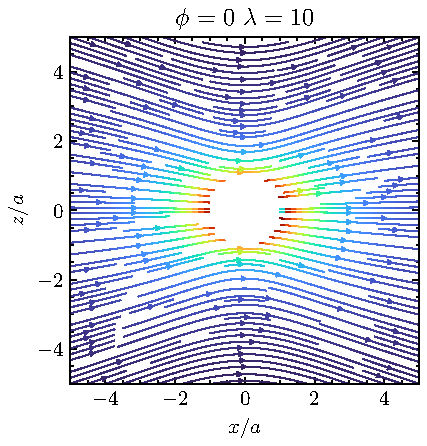
\includegraphics[height = 0.33\textwidth]{image/Vnst_H_l_10_0.pdf}
    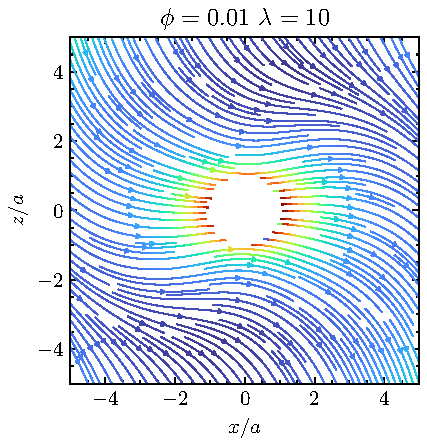
\includegraphics[height = 0.33\textwidth]{image/Vnst_H_l_10_1.pdf}
    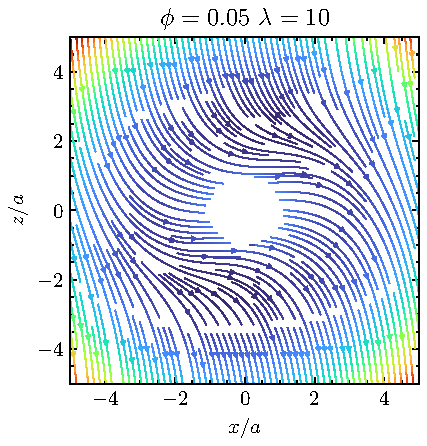
\includegraphics[height = 0.33\textwidth]{image/Vnst_H_l_10_5.pdf}
    % 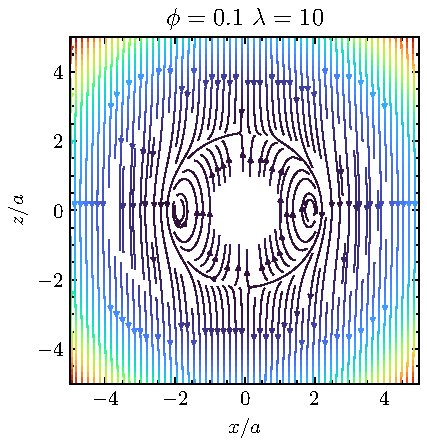
\includegraphics[height = 0.33\textwidth]{image/Vnst_l_10_10.pdf}
    \caption{Streamlines of the disturbance velocity field $\textbf{v}^\text{nst}(\textbf{r}_f)$  \eqref{eq:v_nst_solution_adim} in the cross-section given by the plane $(\textbf{e}_x,\textbf{e}_z)$, for multiples volume fraction $\phi = 0, 0.01$ and $0.05$ at $\lambda = 10$.  
    The color map indicates the magnitude of the velocity, from black which corresponds to a velocity magnitude of 0, to the color at the interface which corresponds to 1.
    In this situation $\textbf{e} = \textbf{e}_x$ and $\textbf{k} = -\textbf{e}_z$.
    The constant $A$ have been arbitrarily set to $1$. }
    \label{fig:vnst_horizontal}
\end{figure}
\end{frame}

\begin{frame}
  {General solution}
  
  \begin{equation*}
    \avg{\chi_f \textbf{u}'_f\textbf{u}'_f}[\textbf{x},t]
    = \phi_f
    \underbrace{\int 
      \textbf{u}^\text{nst}_f
      \textbf{u}^\text{nst}_f 
      P_\text{nst}(\textbf{r}|\textbf{x}) d\textbf{r} 
    }_\text{Averaged wake contribution}
    + \underbrace{ 
      \int \avg{\delta_i h_i \chi_f \textbf{v}_f''\textbf{v}_f''}  d\textbf{r}
    % P_{nst}(\textbf{x},t,\textbf{r}) d\textbf{r}
    }_{\mathcal{O}(\phi^2)}
  \end{equation*}
  \begin{align}
    \frac{\avg{\chi_f \textbf{u}_f'\textbf{u}_f'}}{U^2}
    &= 
    C^{(1)}_e \left[
        \textbf{U}\textbf{U}
        + \frac{\pavg{\textbf{u}_\alpha'\textbf{u}_\alpha'}}{n_p U^2}
         - \frac{1}{3}(\textbf{U}\cdot \textbf{U}+2k_p/U^2)\bm\delta
    \right]
    + C^{(2)}_e 
    (\textbf{U}\cdot \textbf{U}+2k_p/U^2)\bm\delta \nonumber \\
    &+ C^{(1)}_k  \left[
        \textbf{kk}
         - \frac{1}{3}(\textbf{k}\cdot \textbf{k})\bm\delta
    \right]
    +C^{(2)}_k 
    (\textbf{k}\cdot \textbf{k})\bm\delta \nonumber \\
    &+ C^{(1)}_{ek} \left[
        \frac{1}{2}
        (\textbf{U}\textbf{k}  + \textbf{k} \textbf{U})
         - \frac{1}{3}(\textbf{k}\cdot \textbf{U})\bm\delta
    \right]
    + C^{(2)}_{ek}
    (\textbf{U}\cdot \textbf{k})\bm\delta 
\end{align}
% \begin{align*}
%   C_e^{(1)} =
%   % \frac{9(2+3\lambda)^2 \Gamma(\frac{1}{3})}{80(\lambda+1)^2}\phi^{2/3}
%   \frac{27}{10}
%   C_e^{(2)}
%   % + \mathcal{O}(\phi)
%   &&  C_e^{(2)} = \frac{(2+3\lambda)^2 \Gamma(\frac{1}{3})}{24(\lambda+1)^2}\phi^{2/3} \\
%   C_k^{(1)} =
%   3
%   C_k^{(2)}
%   && C_k^{(2)} = A^2 \frac{\Gamma(\frac{7}{3})}{3}\phi^{2/3} \\
%   C_{ek}^{(1)} =
%   3
%   C_{ek}^{(2)}
%   % A\frac{2 (2+3\lambda) \Gamma(\frac{4}{3})}{3 (\lambda+1)}\phi^{2/3}
%   % % + \mathcal{O}(\phi^{4/3})
%   && C_{ek}^{(2)} =
%   A\frac{2 (2+3\lambda) \Gamma(\frac{4}{3})}{9(\lambda+1)}\phi^{2/3}
%   % + \mathcal{O}(\phi^{4/3})
% \end{align*}
$\to$ $\pavg{\textbf{u}_\alpha'\textbf{u}_\alpha'}$ is the variance of the particle  center of mass velocity

$\to$ $k_p  = \frac{1}{2}\pavg{\textbf{u}_\alpha'\cdot\textbf{u}_\alpha'}$ is the variance of the particle  center of mass velocity
\end{frame}

\begin{frame}
  {General solution when $\textbf{U} = -\textbf{k}$}
  \begin{multline}
    \frac{\avg{\chi_f \textbf{u}_f'\textbf{u}_f'}}{U^2}
    = 
    \underbrace{C^{(1)}_e \left[
        \textbf{U}\textbf{U}
        + \frac{\pavg{\textbf{u}_\alpha'\textbf{u}_\alpha'}}{n_p U^2}
         - \frac{1}{3}(\textbf{U}\cdot \textbf{U}+2k_p/U^2)\bm\delta
    \right]}_\text{deviatoric part}\\
    + 
    \underbrace{ C^{(2)}_e  (\textbf{U}\cdot \textbf{U}+2k_p/U^2)\bm\delta}_\text{Isotropic part}
    % &+ C^{(1)}_k  \left[
    %     \textbf{kk}
    %      - \frac{1}{3}(\textbf{k}\cdot \textbf{k})\bm\delta
    % \right]
    % +C^{(2)}_k 
    % (\textbf{k}\cdot \textbf{k})\bm\delta \nonumber \\
    % &+ C^{(1)}_{ek} \left[
    %     \frac{1}{2}
    %     (\textbf{e}_p\textbf{k}  + \textbf{k} \textbf{e}_p)
    %      - \frac{1}{3}(\textbf{k}\cdot \textbf{e}_p)\bm\delta
    % \right]
    % + C^{(2)}_{ek}
    % (\textbf{e}_p\cdot \textbf{k})\bm\delta 
\end{multline}
\begin{align*}
  C_e^{(1)} =
  % \frac{9(2+3\lambda)^2 \Gamma(\frac{1}{3})}{80(\lambda+1)^2}\phi^{2/3}
  \frac{27}{10}
  C_e^{(2)}
  % + \mathcal{O}(\phi)
  &&  C_e^{(2)} = \frac{(2+3\lambda)^2 \Gamma(\frac{1}{3})}{24(\lambda+1)^2}\phi^{2/3} \\
  % C_k^{(1)} =
  % 3
  % C_k^{(2)}
  % && C_k^{(2)} = A^2 \frac{\Gamma(\frac{7}{3})}{3}\phi^{2/3} \\
  % C_{ek}^{(1)} =
  % 3
  % C_{ek}^{(2)}
  % A\frac{2 (2+3\lambda) \Gamma(\frac{4}{3})}{3 (\lambda+1)}\phi^{2/3}
  % % + \mathcal{O}(\phi^{4/3})
  % && C_{ek}^{(2)} =
  % A\frac{2 (2+3\lambda) \Gamma(\frac{4}{3})}{9(\lambda+1)}\phi^{2/3}
  % + \mathcal{O}(\phi^{4/3})
\end{align*}
\begin{enumerate}
  \item $\Gamma(a) = \int_0^\infty t^{a-1} e^{-t} dt $ is the gamma  function. 
  \item  Note that $\lim_{\phi \to 0} \avg{\chi_f \textbf{u}'_f\textbf{u}'_f}(\textbf{x},t)/\phi \sim\phi^{-1/3} =\infty$. 
  \item We found that $\avg{\chi_f \textbf{u}'_f\textbf{u}'_f}(\textbf{x},t)\sim\phi^{2/3}$.  
\end{enumerate}
\end{frame}

% \begin{frame}
%   \frametitle{Stokes flow solution with NPS}
%   \begin{small}
%     \begin{equation*}
%       \textbf{u}_\text{stokes} 
%       = \left(\frac{ \textbf{I}}{r} + \frac{\textbf{rr}}{r^3}\right)  \frac{1}{4}\left(\frac{3\lambda + 2}{\lambda +1}\right) a \textbf{U}
%       - \left(-\frac{\textbf{I}}{r^3} + \frac{3 \textbf{rr} }{r^5}\right)  \frac{1}{4}\left(\frac{\lambda}{\lambda +1}\right) a^3 \textbf{U}
%     \end{equation*}
%   \end{small}
%   In the dilute regime we can write $\textbf{u}_f^\text{nst} = \textbf{u}_\text{stokes}$ thus,  :
%   \begin{equation*}
%     \avg{\chi_f \textbf{u}'_f\textbf{u}'_f}(\textbf{x},t)
%     = 
%     {\int \textbf{u}_\text{stokes} \textbf{u}_\text{stokes}  
%     P_\text{nst}(r) d\textbf{r} }
%     + \mathcal{O}(\phi^2)
%   \end{equation*}\pause
%   \begin{equation*}
%     % - \phi_f \textbf{u}_f\textbf{u}_f\\
%     \boxed{
%     \begin{aligned}
%     &=  \frac{(2+3\lambda)^2\Gamma(1/3)}{80(\lambda+1)^2}\left(
%       9 \textbf{UU}
%       + \frac{1}{3}U^2 \textbf{I}
%     \right)\phi^{2/3}\\
%     &- 
%     \frac{1}{20(\lambda+1)^2}\left[
%       (27+82\lambda + 62\lambda^2) \textbf{UU}
%       + (1+6\lambda + 6\lambda^2) U^2 \textbf{I}
%     \right]\phi+ \mathcal{O}(\phi^2)
%     \end{aligned}
%     }
%     % \left(\frac{9(2+3\lambda)^2 \Gamma(1/3)}{80 (\lambda +1)^2}\phi^{2/3} 
%     % - \frac{27+82\lambda + 62\lambda^2}{20(\lambda + 1)^2}\phi \right)\textbf{UU}\\
%     % + \left(\frac{(2+3\lambda)^2 \Gamma(1/3)}{240 (\lambda +1)^2}\phi^{2/3} 
%     %  - \frac{1+6\lambda + 6\lambda^2}{20(\lambda + 1)^2}\phi \right)U^2\textbf{I} 
%   \end{equation*}
%   \begin{itemize}
%     % \item  \textbf{Hypothesis 1} :$P_\text{nst}(\textbf{r}|\textbf{x}) = \frac{3\phi}{4\pi}
%     % e^{ - \phi (r^3 - 1) }$
%     % \item \textbf{Hypothesis 2} : We considered $\textbf{u}^\text{nst} = \textbf{u}_\text{stokes}$ since it is equivalent in the dilute regime
%     \item Thanks to the fast decay of $P_\text{nst} \sim e^{-\phi (r^3-1)}$ the integral converges ! 
%   \end{itemize}
%   \begin{enumerate}
%     \item $\Gamma(a) = \int_0^\infty t^{a-1} e^{-t} dt $ is the gamma  function. 
%     \item  Note that $\lim_{\phi \to 0} \avg{\chi_f \textbf{u}'_f\textbf{u}'_f}(\textbf{x},t)/\phi \sim\phi^{-1/3} =\infty$. 
%     \item We found that $\avg{\chi_f \textbf{u}'_f\textbf{u}'_f}(\textbf{x},t)\sim\phi^{2/3}$.  
%   \end{enumerate}
    
% \end{frame}

\section{Comparison with DNS and experiment}

\section*{}
\begin{frame}
\frametitle{Direct Numerical Simulation of buoyant emulsions}
\begin{columns}
  \column{0.6\textwidth}
\underline{Simulation set up :} 
\begin{itemize}
  \item Tri -periodic boundary conditions. 
  \item Mono-disperse distribution of droplets size.
  \item We prevent coalesce by the use of a special algorithm 
  (\href{http://basilisk.fr/sandbox/fintzin/Rising-Suspension/no-coalescence.h}{no-coalescence.h})
  \item Free software : \url{https://basilisk.fr}
  \item Simulation source code : \url{http://basilisk.fr/sandbox/fintzin/Rising-suspension/RS.c}
\end{itemize}

\begin{figure}
  \caption{Snapshot of a simulation with $\phi = 0.01$, $Ga = 75$ $\lambda = 0.1$ and $N_b = 125$. In white : the interfaces, The background color map correspond to the pressure field. The grid represents the different core ($\approx 729$).
  }
\end{figure}
\column{0.5\textwidth}
\centering
\href{file:///work/fintzin/BUBLLES_PROJECT/movies/cut.gif}{\beamergotobutton{Play}}
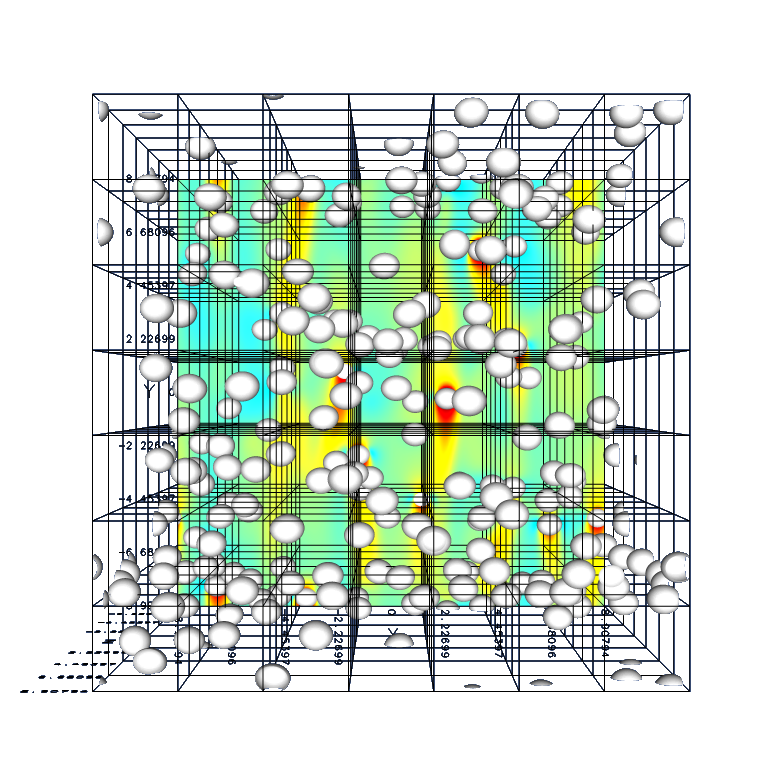
\includegraphics[width =  1.1\textwidth]{image/PHI_01_Ga_75.png}
\end{columns}
\end{frame}

\begin{frame}
  \frametitle{Direct Numerical Simulation of buoyant emulsions}
  \begin{columns}
    \column{0.6\textwidth}
  \underline{Dimensionless parameters :} 
  \begin{itemize}
    \item \textit{Galileo} number : $Ga =\frac{\sqrt{\rho \Delta\rho g(2a)^3}}{\mu} \in [5, 100]$
    \item \textit{Bond} number : $Bo = \frac{\Delta \rho g (2a)^2}{\sigma} = 0.5$ 
    \item volume fraction of dispersed phase : $\phi = [0.01;0.2]$. 
    \item Density and viscosity ratio, $\rho_r=1.11$ and $\lambda= 0.1, 1, 10$. 
  \end{itemize}
  
  \begin{figure}
    \caption{Snapshot of a simulation for $\phi = 0.01$, $Ga = 75$ $\lambda = 0.1$ and $N_b = 125$. In white : the interfaces, The background color map correspond to the pressure field. The grid represents the different core ($\approx 729$).
    }
  \end{figure}
  \column{0.5\textwidth}
  \centering
  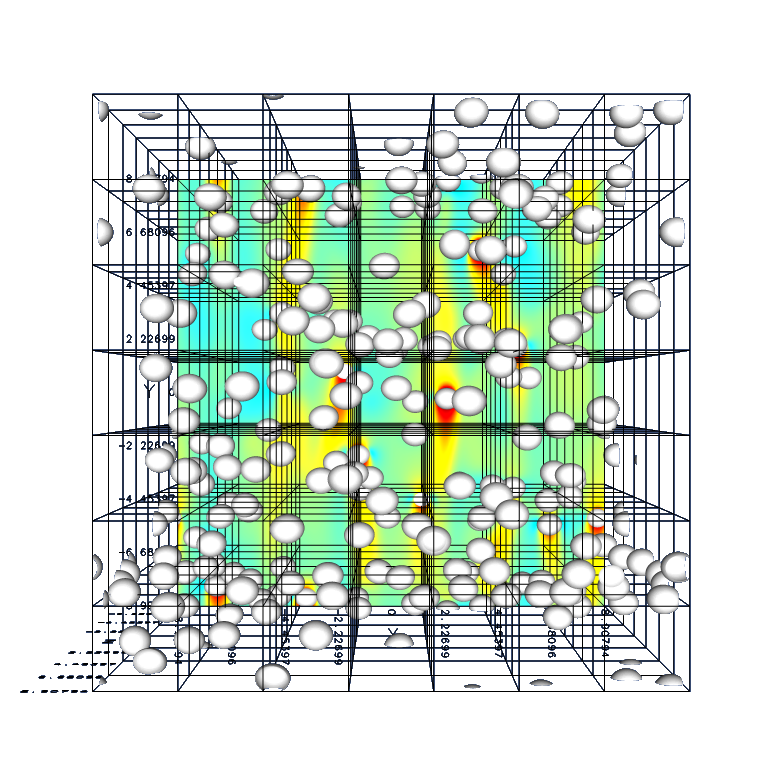
\includegraphics[width =  1.1\textwidth]{image/PHI_01_Ga_75.png}
  \end{columns}
\end{frame}


% \begin{frame}
%   \frametitle{Reconstruction of the velocity fields from DNS}
%   \begin{figure}[h!]
%     \centering
%     \begin{tikzpicture}
%         \node (img) at (0,0)  {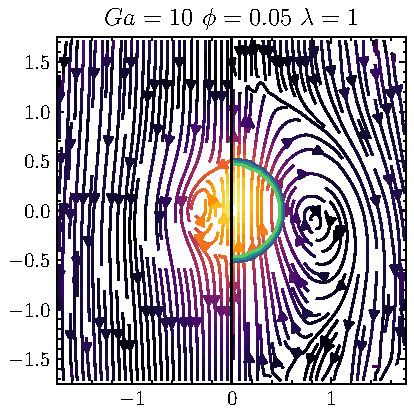
\includegraphics[height=0.25\textwidth]{image/HOMOGENEOUS/Stream/Stream_PHI_5_Ga_10_l_1.pdf}};
%         \node (img) at (0.25\textwidth,0)  {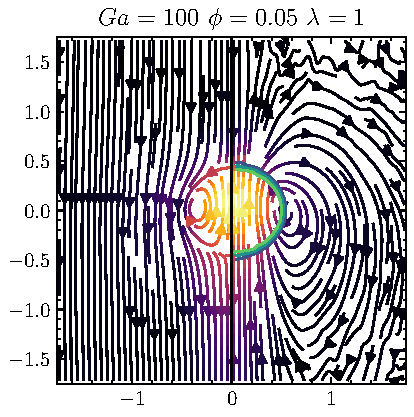
\includegraphics[height=0.25\textwidth]{image/HOMOGENEOUS/Stream/Stream_PHI_5_Ga_100_l_1.pdf}};
%         \node (img) at (0.5\textwidth,0)  {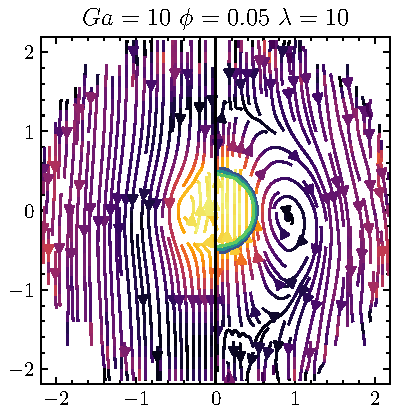
\includegraphics[height=0.25\textwidth]{image/HOMOGENEOUS/Stream/Stream_PHI_5_Ga_10_l_10.pdf}};
%         \node (img) at (0.75\textwidth,0)  {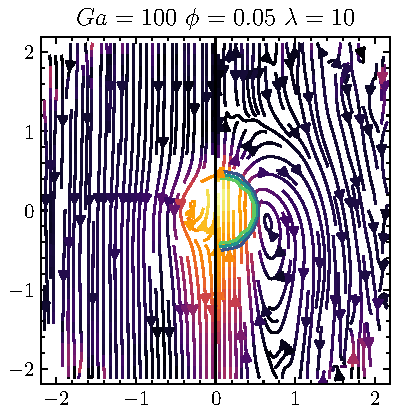
\includegraphics[height=0.25\textwidth]{image/HOMOGENEOUS/Stream/Stream_PHI_5_Ga_100_l_10.pdf}};
%     \end{tikzpicture}
%     \caption{Nearest particle averaged velocity $\nstavg{\textbf{u}}(\textbf{r})$ for  $\phi = 5\%$ and $20\%$.
%     Green lines : contour plots of the nearest averaged indicator function $\nstavg{\chi_d}(\textbf{r})$ (it represent the mean shape of the particles)}
%     \label{fig:Stream}
%   \end{figure}
  
%   \begin{itemize}
%     \item Close from the drop ($r=\mathcal{O}(a)$) we can see that $\textbf{u}_\text{nst} \approx \textbf{u}_\text{stokes}$. 
%   \end{itemize}
% \end{frame}

% \begin{frame}
%   \frametitle{Nearest particle statistic solution for translating drops in stokes flow :}
%   \begin{multline}
%     \avg{\chi_f \textbf{u}'_f\textbf{u}'_f}(\textbf{x},t)
%     = 
%     {\int_a^\infty \textbf{u}_\text{stokes} \textbf{u}_\text{stokes}  P_{nst}(\textbf{x},t,\textbf{r}) d\textbf{r} }
%     - \phi_f \textbf{u}_f\textbf{u}_f
%     \\=
% -\left({{-\left(9\,\Gamma\left(-1 , \,\phi\right)\,\lambda^2\,\phi
% ^{{{4}\over{3}}}\,e^{\phi}\right)+\ldots}\over{\left(120\,\lambda^2+240\,\lambda+
% 120\right)\,\phi^{{{1}\over{3}}}}}\right)
% \textbf{e}_U\textbf{e}_U + \ldots
% \end{multline}
% \begin{itemize}
%   \item $\textbf{e}_U$ is the units vector in the direction of the drift velocity. 
% \end{itemize}

% \end{frame}

\begin{frame}
  \frametitle{Comparison with DNS}
  \begin{figure}
    \centering
    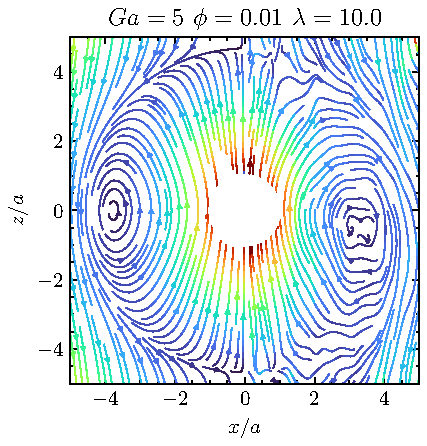
\includegraphics[width = 0.32\textwidth]{image/HOMOGENEOUS_final/Stream/Stream_PHI_1_Ga_5_l_10.pdf}
    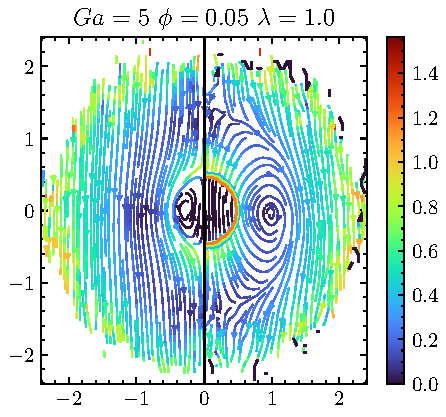
\includegraphics[width = 0.32\textwidth]{image/HOMOGENEOUS_final/Stream/Stream_PHI_5_Ga_5_l_10.pdf}
    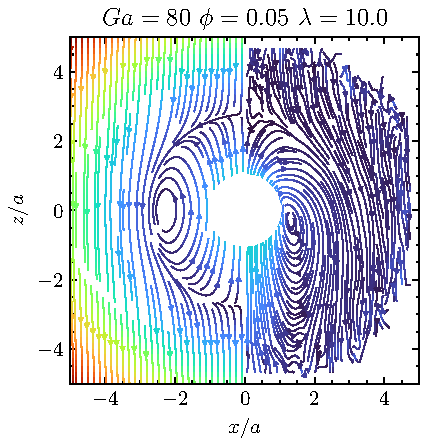
\includegraphics[width = 0.32\textwidth]{image/HOMOGENEOUS_final/Stream/Stream_PHI_5_Ga_80_l_10.pdf}
    \caption{\footnotesize
      Streamlines of the disturbance velocity field $\textbf{v}^\text{nst}$, in the cross-section given by the plane $(\textbf{e}_x,\textbf{e}_z)$, for two volume fractions $\phi = 0.01$ (left) and $\phi = 0.05$ (middle) at $\lambda = 10$ and $Ga = 5$.
    (right) plot of the inertial case $Ga = 80$. 
    The left side of the panel ($x/a < 0$), we have re-plotted the theoretical solution provided by \ref{eq:v_nst_solution_adim}.   
    The right side of the panel ($x/a > 0$), we have reconstructed the streamlines obtained with the DNS, using \ref{eq:vnst_DNS}. 
    The color map indicates the magnitude of the velocity, from black which corresponds to a velocity magnitude of 0, to the color at the interface of the droplet which corresponds to a magnitude of 1.}
    \label{fig:vnst_DNS}
\end{figure}
\end{frame}

  \begin{frame}
  \frametitle{Comparison with DNS results and experiments}
  \begin{figure}[h!]
    \centering    
    % 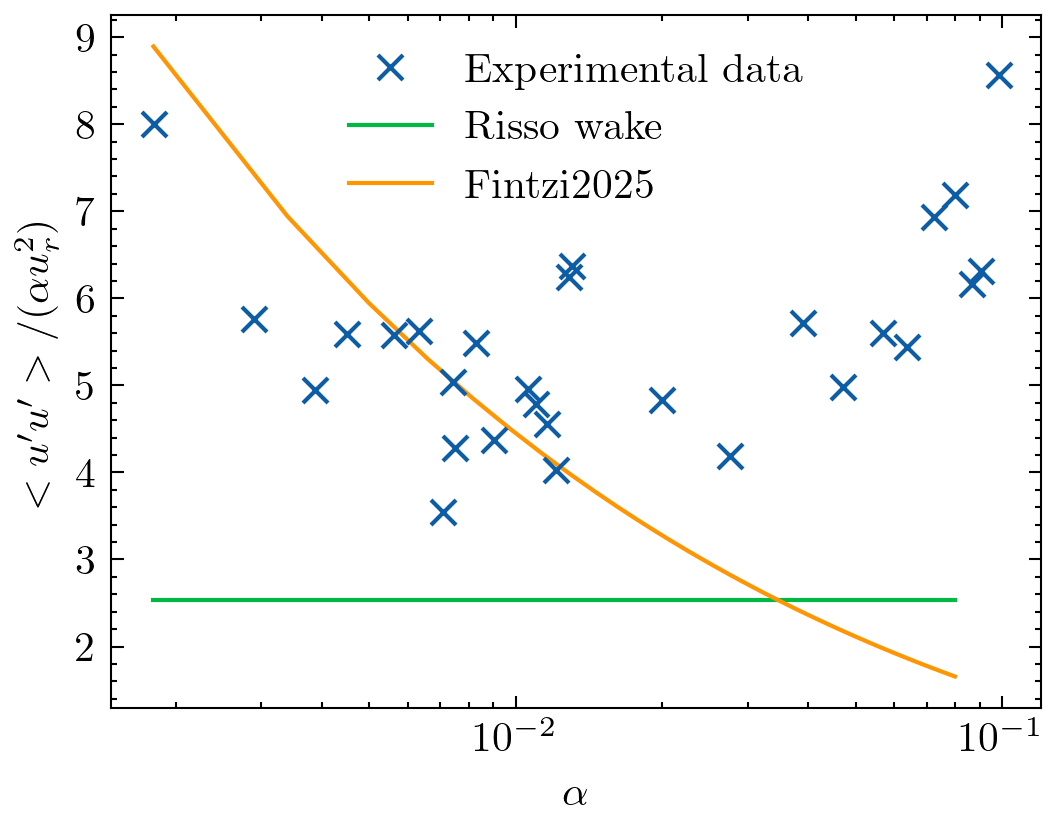
\includegraphics[height = 0.25\textwidth]{image/upupexp.png}
    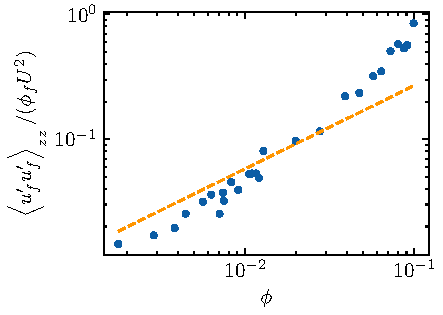
\includegraphics[height = 0.25\textwidth]{image/HOMOGENEOUS_final/CA/cartellier.pdf}
    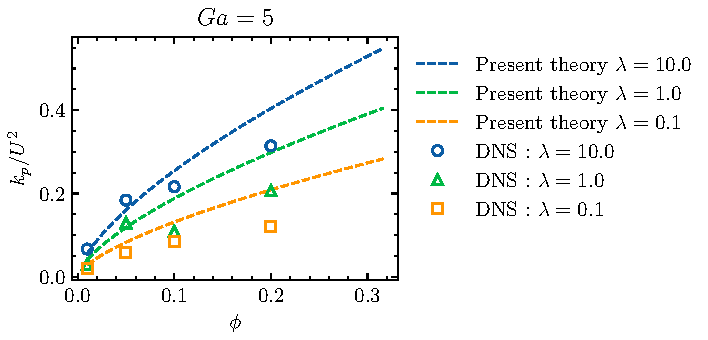
\includegraphics[height = 0.25\textwidth]{image/HOMOGENEOUS_final/CA/UUyy_Ga_5.pdf}
    \caption{
       Dimensionless vertical component of the Reynolds stress :
       (left) Comparison with the rising bubbles experiment of Cartellier (2009) with $Re \approx 10$. 
       (right) comparison with DNS for two viscosity ratio $\lambda =1,10$ and $Re \approx 1$ DNS. 
    }
    \label{fig:Cp}
\end{figure}  
\begin{itemize}
  \item Good trends in terms of $\phi$ and $\lambda$.  
  \item Quantitative agreement for $\phi < 0.01$.  
\end{itemize}
\end{frame}

\begin{frame}
  \frametitle{Extension to finite inertial numbers}
  \begin{figure}
    \centering
    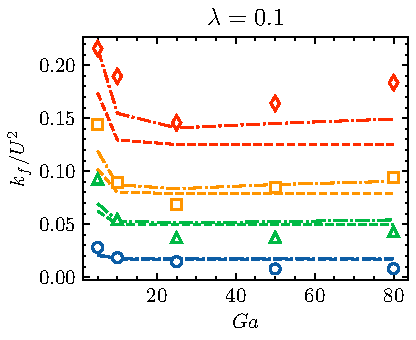
\includegraphics[height = 0.25\textwidth]{image/HOMOGENEOUS_final/CA/KF2_l_0.pdf}
    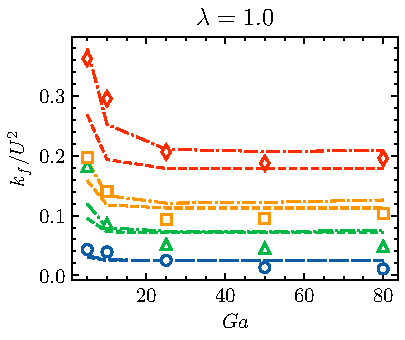
\includegraphics[height = 0.25\textwidth]{image/HOMOGENEOUS_final/CA/KF2_l_1.pdf}
    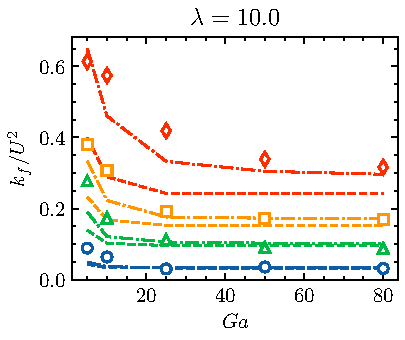
\includegraphics[height = 0.25\textwidth]{image/HOMOGENEOUS_final/CA/KF2_l_10.pdf}
    \caption{\footnotesize
      Dimensionless continuous phase pseudo turbulent energy, $k_f/U^2$ in terms of the \textit{Galileo} number.
    (left) $\lambda = 0.1$
    (middle) $\lambda = 1$
    (right) $\lambda = 10$
    (Symbols) DNS results. 
    ($\pmb\bigcirc$) $\phi = 0.01$; ($\pmb\triangle$) $ \phi = 0.05$; ($\pmb\square$) $\phi = 0.1$ ($\pmb\lozenge$) $\phi = 0.2$.
    (dot-dashed lines) Semi-empirical formula (\ref{eq:semi_empirical}) \underline{including} the results of the DNS for the particle phase velocity fluctuations. 
    (dashed lines) Semi-empirical formula (\ref{eq:semi_empirical}) \underline{excluding} the particle phase velocity fluctuations. 
    }
    \label{fig:kf}
\end{figure}
\begin{equation}
  k_f
  = 
  \underbrace{C_e^{(0)}  \left( U^2 + 2 k_p\right)  \frac{3}{2}}_\text{Theoritical solution}
  \underbrace{\frac{1}{2}\left(e^{-Re} +1\right)}_{\text{empirical factor}}.
  \label{eq:semi_empirical}
\end{equation}

\end{frame}


\begin{frame}
  \frametitle{Validation at higher inertial effects }

  \begin{figure}
    \centering
    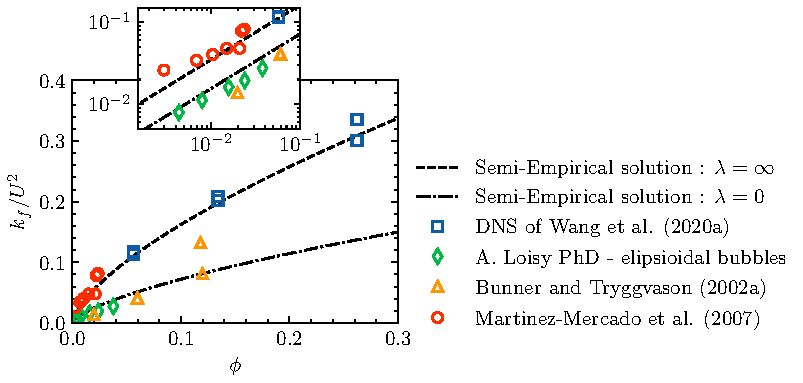
\includegraphics[height = 0.35\textwidth]{image/HOMOGENEOUS_final/CA/KFliterature.pdf}
    \caption{\footnotesize
      Dimensionless continuous phase pseudo turbulent energy, $k_f/U^2$ in terms of the \textit{Galileo} number.
    (Symbols) DNS and experimental results of: 
    ($\pmb\square$)  Particle-resolved Direct Numerical Simulations (PR-DNS)
    of fixed solid spherical particle assemblies at $20< Re < 100$  by \citet{wang2021numerical}; 
    ($\pmb\lozenge$) Direct numerical simulation (DNS) of rising deformable bubbles at $Re \approx 30$ \citep{loisy2016direct}
    ($\pmb\triangle$) DNS of rising spherical bubbles by \citet{bunner2002dynamics}. 
    ($\pmb\bigcirc$) Experiment of rising spherical bubbles in water by \citet{martinez2007measurement} at $Re \approx 30$. 
    (dot-dashed lines) Semi-empirical formula (6) at $Re \approx 30$ with $\lambda = 0$. 
    (dashed lines)  Semi-empirical formula (6) at $Re \approx 30$ with $\lambda = \infty$.
    }
    \label{fig:trygvason}
\end{figure}

\end{frame}
\begin{frame}
  \frametitle{Validation at higher inertial effects }

  \begin{figure}
    \centering
    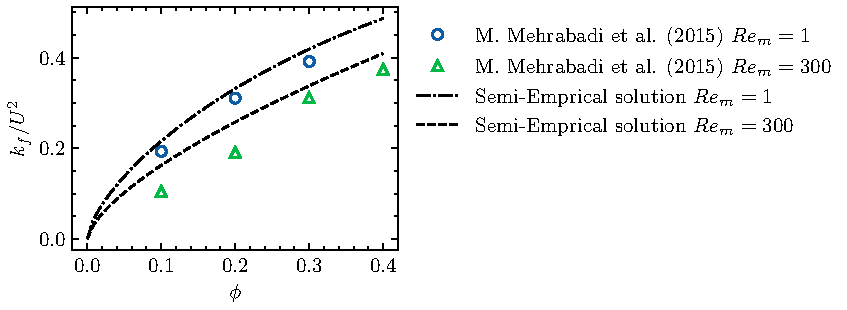
\includegraphics[height = 0.25\textwidth]{image/HOMOGENEOUS_final/CA/tenneti.pdf}
    \caption{Dimensionless continuous phase pseudo turbulent energy, $k_f/U^2$ in terms of the volume fraction $\phi$.
    (Symbols) 
    results of Particle-resolved Direct Numerical Simulations
    of fixed particle assemblies by \citet{mehrabadi2015pseudo}
    ($\pmb\bigcirc$) $Re_m = (1-\phi) \approx 1$; ($\pmb\triangle$) $Re_m \approx 300$;
    (dot-dashed lines) Semi-empirical formula \ref{eq:} at $Re_m = 1$
    (dashed lines) Semi-empirical formula \ref{eq:} at $Re_m= = 300$
    }
    \label{fig:tennet}
\end{figure}

\end{frame}
\begin{frame}
  \frametitle{Validation at higher inertial effects }

  \begin{figure}
    \centering
    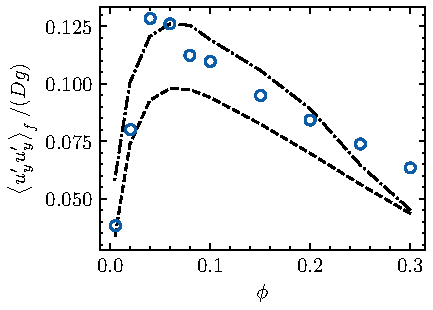
\includegraphics[height = 0.25\textwidth]{image/HOMOGENEOUS_final/CA/tariq.pdf}
    \caption{Dimensionless vertical velocity varience, in terms of the volume fraction $\phi$. 
    (Symbols) results of Particle-resolved Direct Numerical Simulations  of gravitational settling of monodisperse solid spheres by \citet{shajahan2023inertial} at $Ga = 144$. 
    (dot-dashed lines) Semi-empirical formula \underline{including} \citet{shajahan2023inertial}'s results for the particle phase velocity fluctuations. 
    (dashed lines) Semi-empirical formula \underline{excluding} the particle phase velocity fluctuations. 
    }
    \label{fig:tariq}
\end{figure}

\end{frame}
\begin{frame}
  {Going further}
  Toward a more complete model of \textbf{Drops induced turbulence} : 
  \small
  \begin{equation*}
    \avg{\chi_f  \textbf{u}_f' \textbf{u}_f'}
    =
    \underbrace{
      C_1(\phi)\textbf{UU}
    + C_2(\phi)U^2 \textbf{I}
    + \overbrace{C_1(\phi)\avg{\textbf{u}_p'\textbf{u}_p'}
    + C_2(\phi)\avg{\textbf{u}_{p}'\cdot \textbf{u}_{p}'}\textbf{I}
    }^{\text{Particle center of mass velocity fluctuations}}
    }_\text{Particle Induced Turbulence (PIT)}
    % }_\text{Bubble induced turbulence in a uniform flow}
    % \\
  \end{equation*}
  \pause
  \begin{equation*}
    + \underbrace{\frac{\phi_d a^2 }{105 (\lambda +1)^2 }\left[
        (129\lambda^2+108\lambda+24)\textbf{E}\cdot \textbf{E}
        + (20\lambda^2 +20\lambda + 6)
        (\textbf{E} : \textbf{E})\textbf{I}
    \right]}_\text{Shear Particle Induced Turbulence (S-PIT)}
\end{equation*}
\begin{columns}
  \column{0.5\textwidth}
  \begin{itemize}
    \item $\avg{\textbf{u}_p'\textbf{u}_p'}$ Particles center of mass velocity fluctuation.  
    \item $\textbf{E}$ Mean fluid phase shear rate. 
  \end{itemize}
  \begin{align*}
    C_{1} = \left(\frac{9(2+3\lambda)^2 \Gamma(1/3)}{80 (\lambda +1)^2}\phi^{2/3} 
    - \ldots\right)\\
    % C_2 = \left(\frac{9(2+3\lambda)^2 \Gamma(1/3)}{80 (\lambda +1)^2}\phi^{2/3} 
    % - \frac{27+82\lambda + 62\lambda^2}{20(\lambda + 1)^2}\phi \right)
  \end{align*}
  \column{0.2\textwidth}
  \begin{figure}
    \caption{Disturbance velocity field of a droplet immersed in a pure linear flow}
  \end{figure}
  \column{0.4\textwidth}
  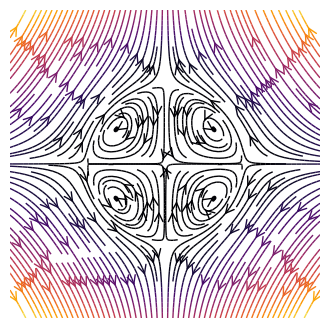
\includegraphics[width=0.6\textwidth]{image/Shear_Stokes.png}
\end{columns}
\end{frame}

% \begin{frame}
%   \frametitle{perspectives}

%   \begin{itemize}
%     \item Compute the Ossen wake contribution to the Reynolds stress. 
%     \item Extend the model validity with DNS results. 
%   \end{itemize}

% \end{frame}

\section{Droplets center of mass velocity variance}

\begin{frame}
  \frametitle{Reformulation of the fluctuation tensor }

  \begin{equation}
    \pavg{\textbf{u}_\alpha'\textbf{u}_\alpha'}
    = 
    n_p[\textbf{x},t]
    \int_{\mathbb{R}^3}
    (\textbf{v}^\text{nst}_p
    \textbf{v}^\text{nst}_p)
    P_\text{nst}
    d\textbf{y}
    + 
    \mathcal{O}(\phi^2)
\end{equation}
\begin{itemize}
  \item $\textbf{u}_\alpha' = \textbf{u}_\alpha - \textbf{u}_p$ relative particle velocity
  \item $P_\text{nst}$ probability of finding a particle center of mass at \textbf{x} with its nearest neighbor at \textbf{y}
  \item $\textbf{v}^\text{nst}_p$ mean center of mass velocity of the particles conditionally on having a nearest neighbor at \textbf{y}. 
\end{itemize}
\end{frame}
\begin{frame}
  \frametitle{Method of reflections}
Velocity field at the point \textbf{x} induced by the nearest neighboring buoyant spherical droplet located at \textbf{y}: 
  \begin{equation}
    \textbf{v}_2 = 
    \underbrace{\textbf{b} \cdot \left[
        1
        + \frac{\lambda}{2(3\lambda +2)}\grad^2
    \right]\frac{\mathcal{G}(\textbf{z},\textbf{y})}{8a\pi\mu_f}}_\text{Wake of an isolated droplet}
    - 
    \underbrace{\phi \frac{\textbf{b}}{4 \pi \mu_f a} |\textbf{z} - \textbf{y}|^2}_\text{Backflow velocity}
\end{equation}
With \textbf{b} the weight of the particle and $\mathcal{G}$ the Ossen tensor. 

\end{frame}
\begin{frame}
  \frametitle{Method of reflections usign Faxen's law}
According to the Faxen law the velocity of a force free droplet immersed in the disturbance field $\textbf{v}_2$ due to a neighboring droplet is, 
\begin{align}
  2 \pi \mu_f a \textbf{v}_p^\text{nst}
  = \left(1 + \frac{\lambda}{2(3\lambda +2)}\grad^2\right)\textbf{v}_2|_{\textbf{z} = \textbf{x}}
\end{align}
\end{frame}

\begin{frame}
  \frametitle{Comparaison with DNS}

  \begin{figure}
    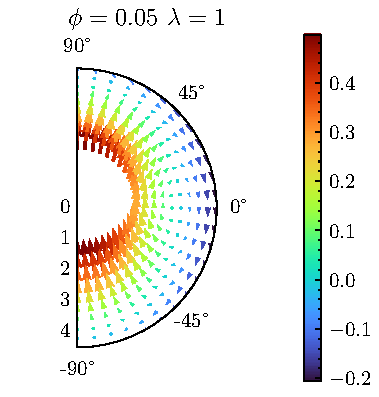
\includegraphics[height = 0.4\textwidth]{image/Vnst_p_l_1_5.pdf}
    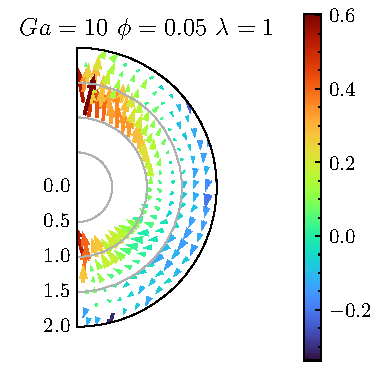
\includegraphics[height = 0.4\textwidth]{image/HOMOGENEOUS_final/Dist/U_l_1_Ga_10_PHI_5.pdf}
    \caption{Theoretical values of $\textbf{v}_p^\text{nst}$, (left) Vs. DNS (right) }
  \end{figure}
  
\end{frame}

\begin{frame}
  \frametitle{The solution }
  \begin{equation*}
    \pavg{\textbf{u}_\alpha'\textbf{u}_\alpha'}
    = 
    n_p[\textbf{x},t]
    \int_{\mathbb{R}^3}
    (\textbf{v}^\text{nst}_p
    \textbf{v}^\text{nst}_p)[\textbf{x},\textbf{y},t]
    P_\text{nst}[\textbf{y}|\textbf{x},t]
    d\textbf{y}
    = 
    C_1[\textbf{UU} - \frac{1}{3}U^2\bm\delta] 
    + C_2U^2\bm\delta
\end{equation*}
\begin{align}
  C_1 = \frac{1}{960}\left(\frac{2+3\lambda}{\lambda+1}\right)^2 \left[
    108\Gamma(1/3)
    - 80\Gamma (4/3)
    +15\Gamma(7/3)
  \right]\phi^{2/3}\\
  C_2 = \frac{1}{576}\left(
    \frac{2+3\lambda}{\lambda+1}\right)^2 \left[
    24\Gamma(1/3)
    - 16\Gamma (4/3)
    +3\Gamma(7/3)
  \right]\phi^{2/3}
\end{align}
  \begin{figure}
    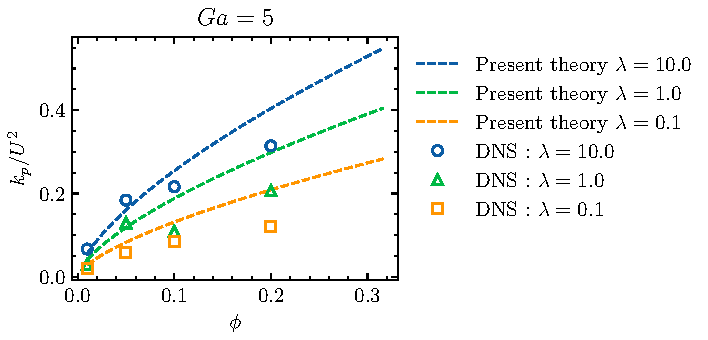
\includegraphics[height = 0.25\textwidth]{image/HOMOGENEOUS_final/CA/UUyy_Ga_5.pdf}
  \end{figure}
\end{frame}
\begin{frame}
  \frametitle{Comparison with experimental results}
\begin{figure}
  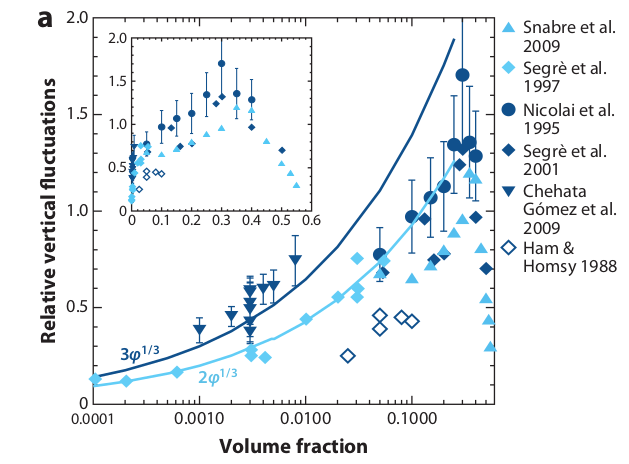
\includegraphics[height = 0.4\textwidth]{image/guazzeli.png}
\end{figure}
  
For solid particle we find $1.52\phi^{1/3}$ instead of $2\phi^{1/3}$ or $3\phi^{1/3}$ so we underestimate the fluctuations. 
This is because this is only a first order approximation. 


\end{frame}
\backmatter
\begin{frame}
  \bibliography{Bib/bib_bulles.bib}

  

\end{frame}
\begin{frame}
  {Going further}
   Model for \textbf{Drops induced dissipation rate} : 
   \begin{multline*}
    \avg{\chi_f \bm\sigma_f^0 :\grad\textbf{u}_f^0}
    =
    \frac{3\mu_f \phi_d}{2a^2}
    \frac{(3\lambda^2 + 4\lambda +2)}{(\lambda + 1)^2}
    (\textbf{u}_{fp}\cdot \textbf{u}_{fp} + 2 \avg{\textbf{u}_p'\cdot\textbf{u}_p'}) \\
    + 
    \frac{3\mu_f \phi_d}{5}
    \frac{(5\lambda^2 + 4\lambda +4)}{(\lambda + 1)^2}
    \textbf{E}:\textbf{E}
    +2 \phi_f \textbf{E}:\textbf{E}
\end{multline*}
\end{frame}

\begin{frame}
  \frametitle{Potential flow solution with NPS}
  In the dilute regime we can write 
  \begin{multline*}
    \avg{\chi_f \textbf{u}'_f\textbf{u}'_f}(\textbf{x},t)
    = 
    {\int \textbf{u}_\text{pot} \textbf{u}_\text{pot}  
    P_\text{nst}(r) d\textbf{r} }
    % - \phi_f \textbf{u}_f\textbf{u}_f\\
    =  \left(\frac{3}{20} U^2\textbf{I} + \frac{1}{20}\textbf{UU} \right)
    \underline{\Gamma_\text{inc}(-1,\phi)\phi^2 e^\phi}
  \end{multline*}

  \begin{itemize}
    \item  \textbf{Hypothesis 1} :$P_\text{nst}(\textbf{r}|\textbf{x}) = \frac{3\phi}{4\pi}
    e^{ - \phi (r^3 - 1) }$
    \item \textbf{Hypothesis 2} : We considered $\textbf{u}^\text{nst} = \textbf{u}_\text{potential}$ since it is equivalent in the dilute regime
    \item $\Gamma_\text{inc}(a,x) = \int_x^\infty t^{a-1} e^{-t} dt $ is the incomplete gamma  function. 
  \end{itemize}

  $\to$ Note that $\Gamma_\text{inc}(-1,\phi)\phi^2 e^\phi \approx  \phi + \mathcal{O}(\phi^2)$ Therefore, we recover  Wijngaarden(1976) solution ! 

\end{frame}


\begin{frame}
  \frametitle{Comparison with DNS results and experiments}
  \begin{figure}[h!]
    \centering    
    % 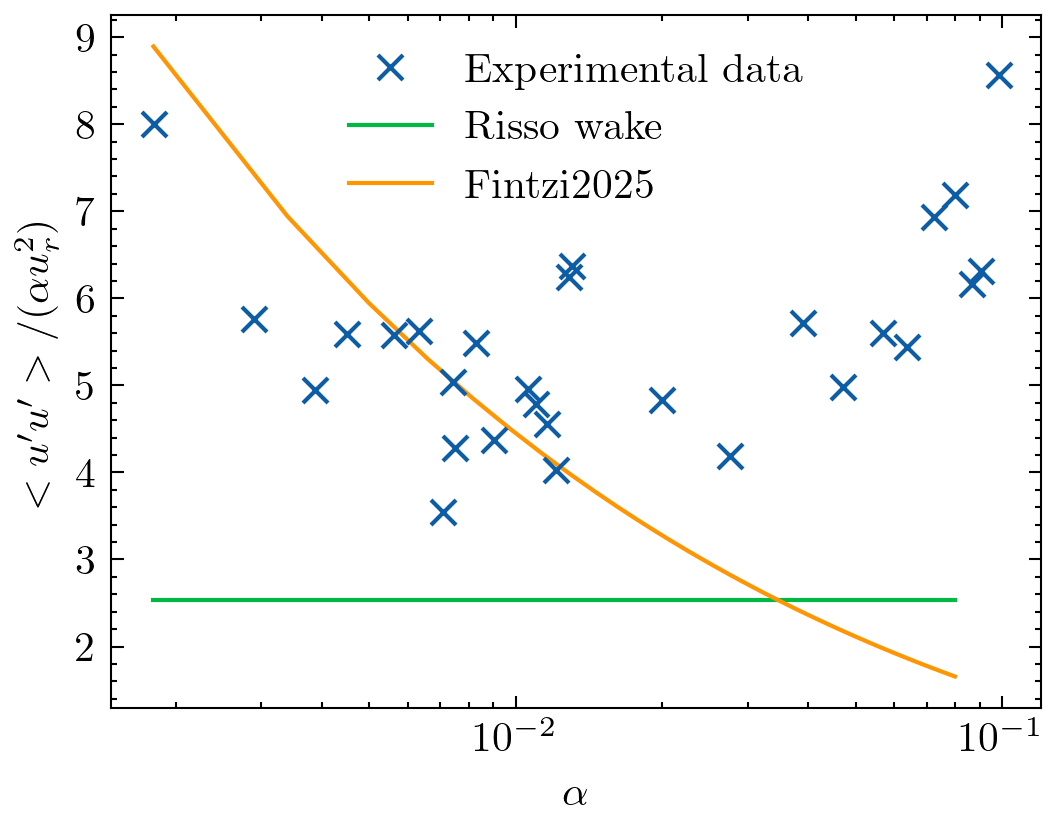
\includegraphics[height = 0.25\textwidth]{image/upupexp.png}
    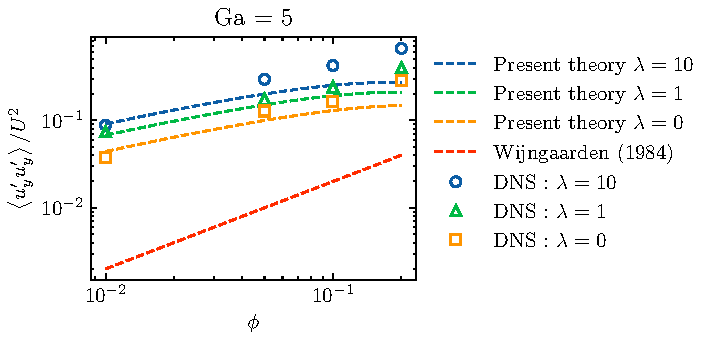
\includegraphics[height = 0.25\textwidth]{image/HOMOGENEOUS_NEW/CA/UUyy.pdf}
    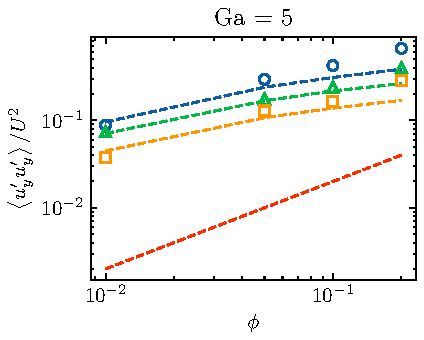
\includegraphics[height = 0.25\textwidth]{image/HOMOGENEOUS_NEW/CA/UUyykp.pdf}
    \caption{
       Dimensionless vertical component of the Reynolds stress :
       (left) Without the contribution from the particle phase velocity fluctuation . 
       (left) Including the contribution from the particle phase velocity fluctuation . 
    }
    \label{fig:Cp}
\end{figure}  
\begin{itemize}
  \item A slight improvement is observed
\end{itemize}
\end{frame}



\end{document}

